\documentclass[12pt, a4paper]{article}
\usepackage[utf8]{inputenc}
\usepackage[russian]{babel}
\usepackage[pdftex]{graphicx, color}
\usepackage{amsmath, amsfonts, amssymb, amsthm}
\usepackage[left=2cm,right=2cm,top=1.5cm,bottom=2cm]{geometry}
\usepackage{indentfirst}

\usepackage{setspace}
\onehalfspacing
\graphicspath{{pics/}}

\begin{document}

    \thispagestyle{empty}

    \begin{singlespace}
    \begin{titlepage}
        \begin{center}
            
\includegraphics[height = 3cm]{msu.png}

            {\scshape Московский государственный университет имени М.~В.~Ломоносова}\\
            Факультет вычислительной математики и кибернетики\\
            Кафедра математических методов прогнозирования\\
            \centerline{\hfill\hrulefill\hrulefill\hrulefill\hrulefill\hfill}

            \vfill

            {\LARGE Отчет к практическому заданию \textnumero 4 по МОМО: \\ Минимизация суммы функций}

            \vspace{1cm}

        \end{center}

        \vfill

        \begin{flushright}
            Студент 517 группы:\\
                \textit{Оспанов А.М.}

            \vspace{5mm}

        \end{flushright}

        \vfill

        \begin{center}
            Москва, 2016
        \end{center}
    \end{titlepage}
    \end{singlespace}

    \newpage


    \section{Введение}
    В данной работе будут реализованы и протестированы два популярных метода для минимизации суммы функций:
    SGD (Stochastic Gradient Descent) и SVRG (Stochastic Variance Reduced Gradient).

    Тестирование будет проводится на следующих двух моделях из области машинного обучения: 1) логистическая регрессия; 2) автокодировщик (глубокая нейронная сеть)

    Код написан на языке Python 3 с использованием библиотеки numpy.

    \section{SGD (Stochastic Gradient Descent)}
    \subsection{Зависимость скорости сходимости от длины шага}
    Запустим метод для модели логистической регрессии.

    На данных w5a видно, что, чем больше шаг, тем быстрее сходится метод

    \def \picwidth {17cm}
    \begin{center}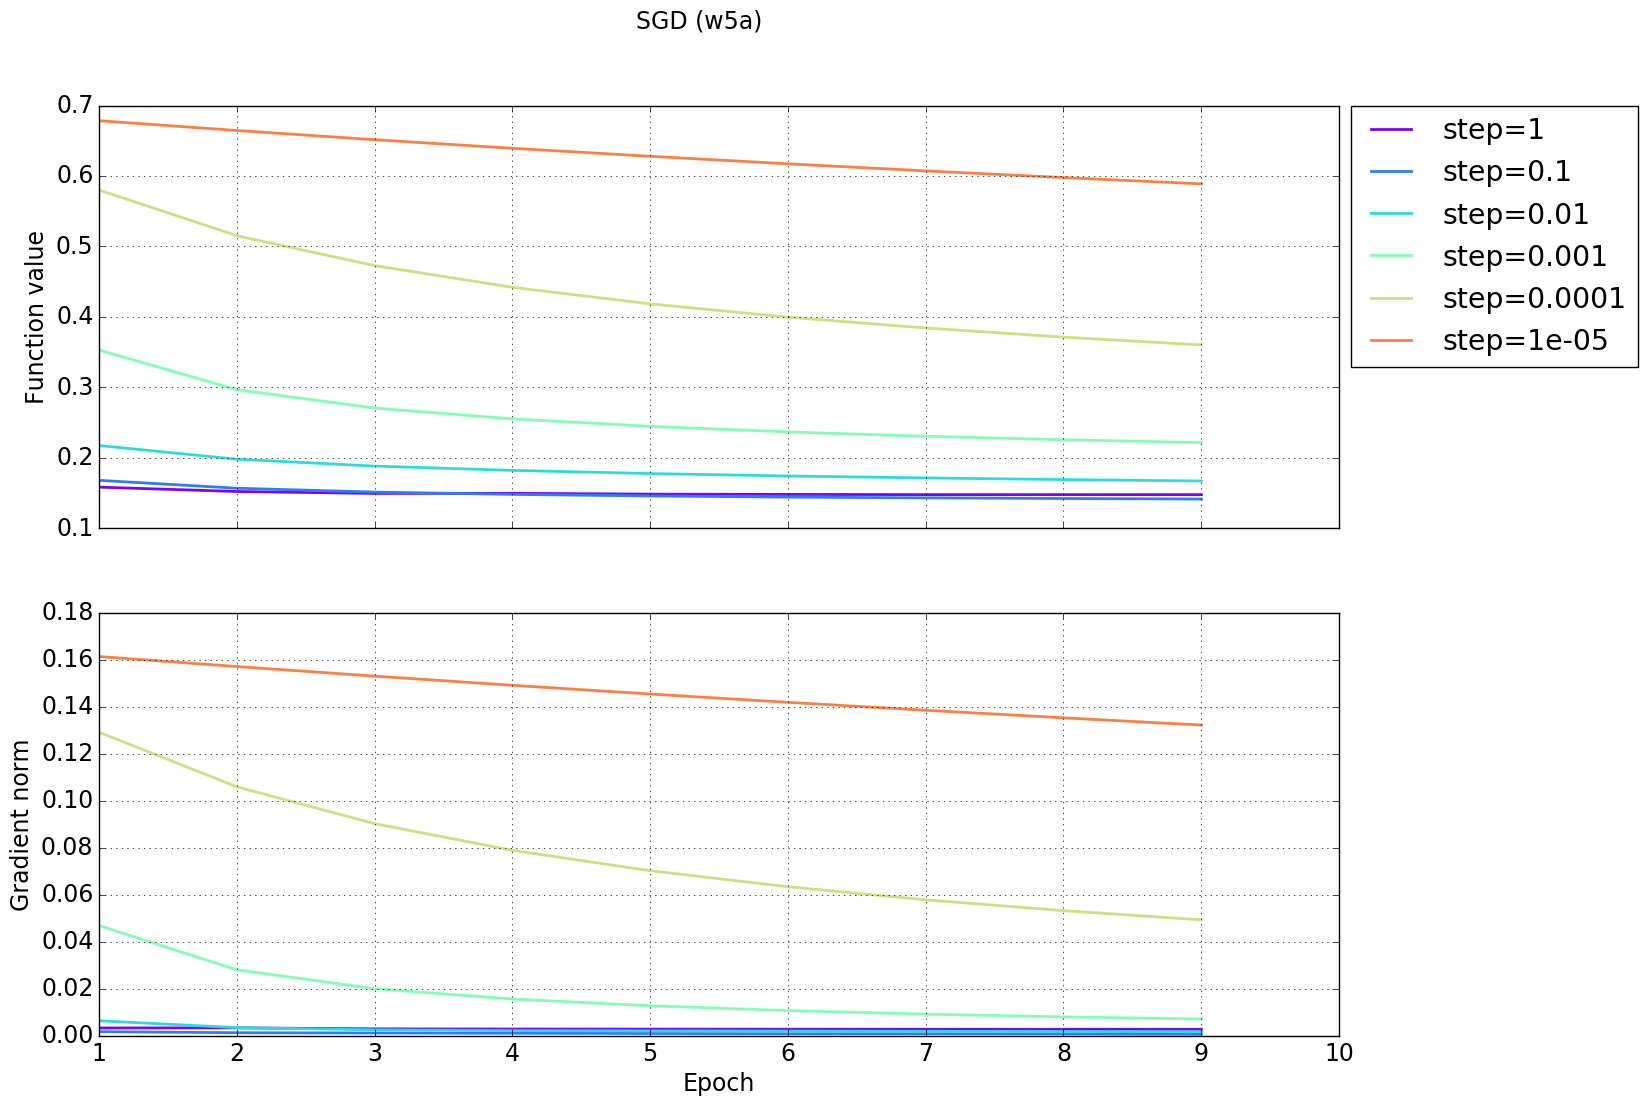
\includegraphics[width=\picwidth]{sgd_w5a.png}\end{center}

    Посмотрим в увеличенном варианте графика. Тут хорошо видно, что при шаге 0.1, метод сходится быстрее. Т.е. пока будем считать, что выбрали шаг = 0.1.

    \begin{center}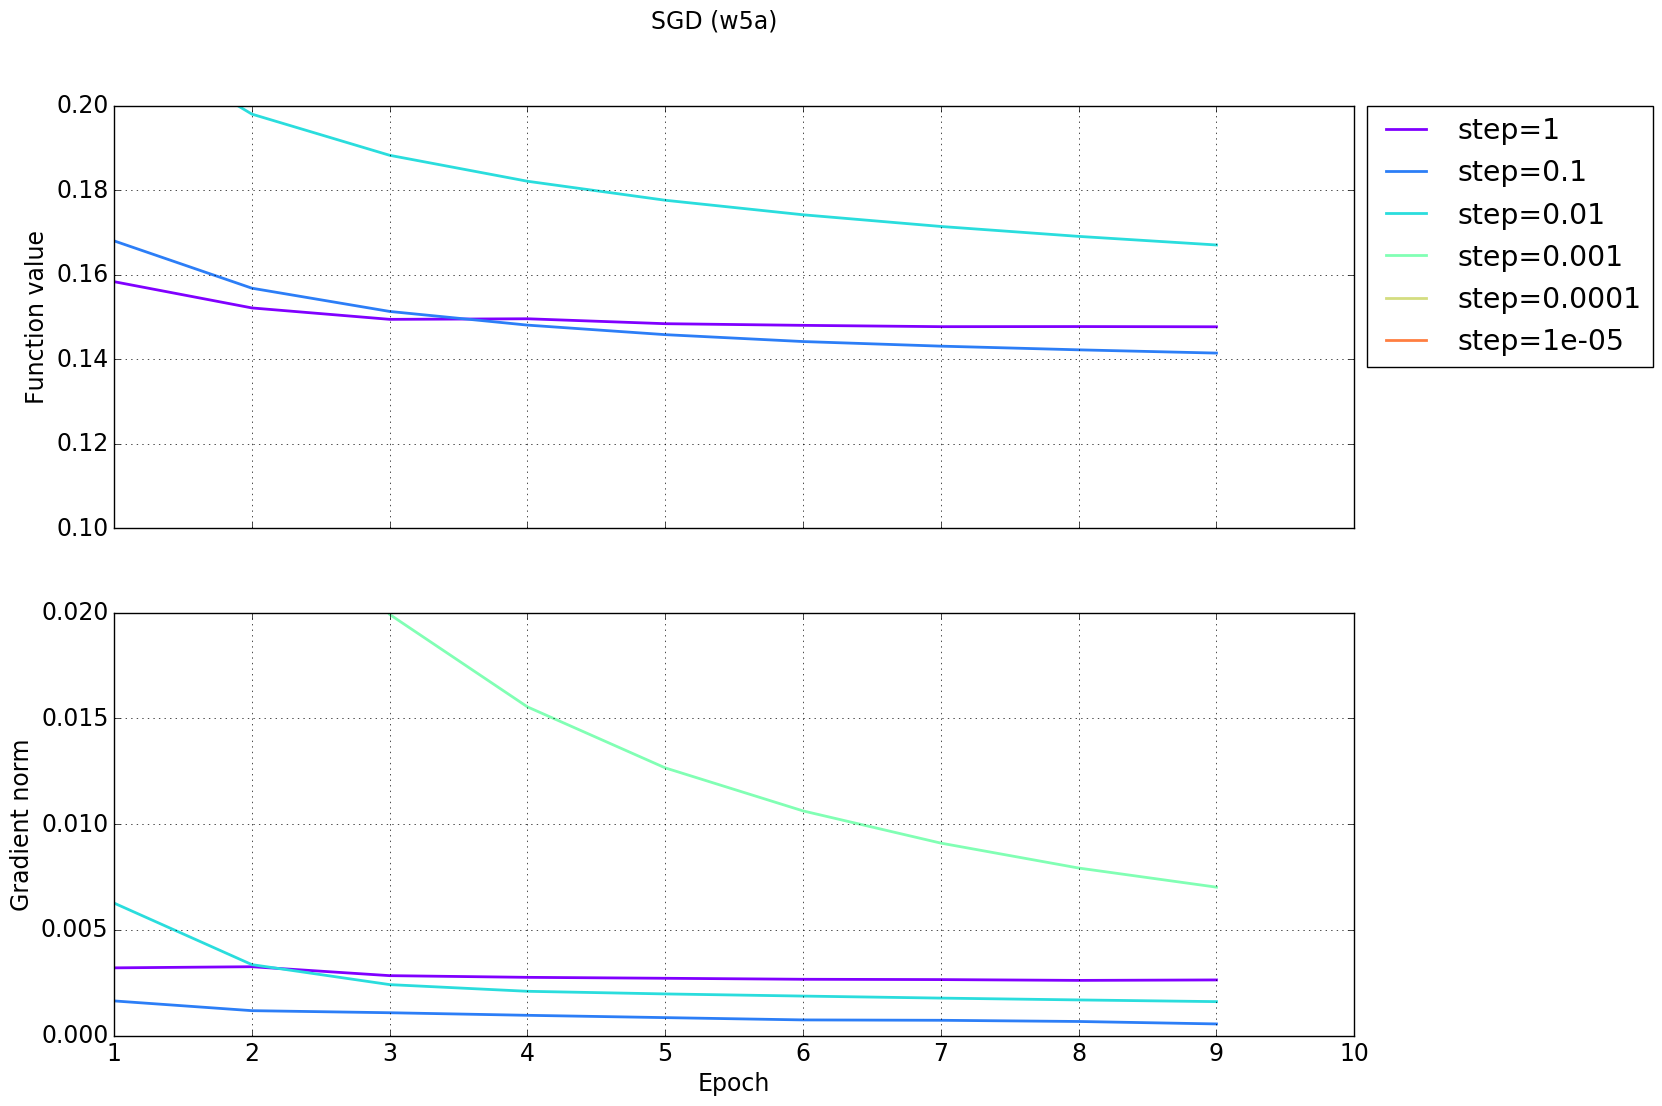
\includegraphics[width=\picwidth]{sgd_w5a_zoomed.png}\end{center}

    Далее посмотрим график для данных a9a. Тут примерно тот же случай, что и с w5a, и чем больше шаг, тем быстрее метод сходится.

    \begin{center}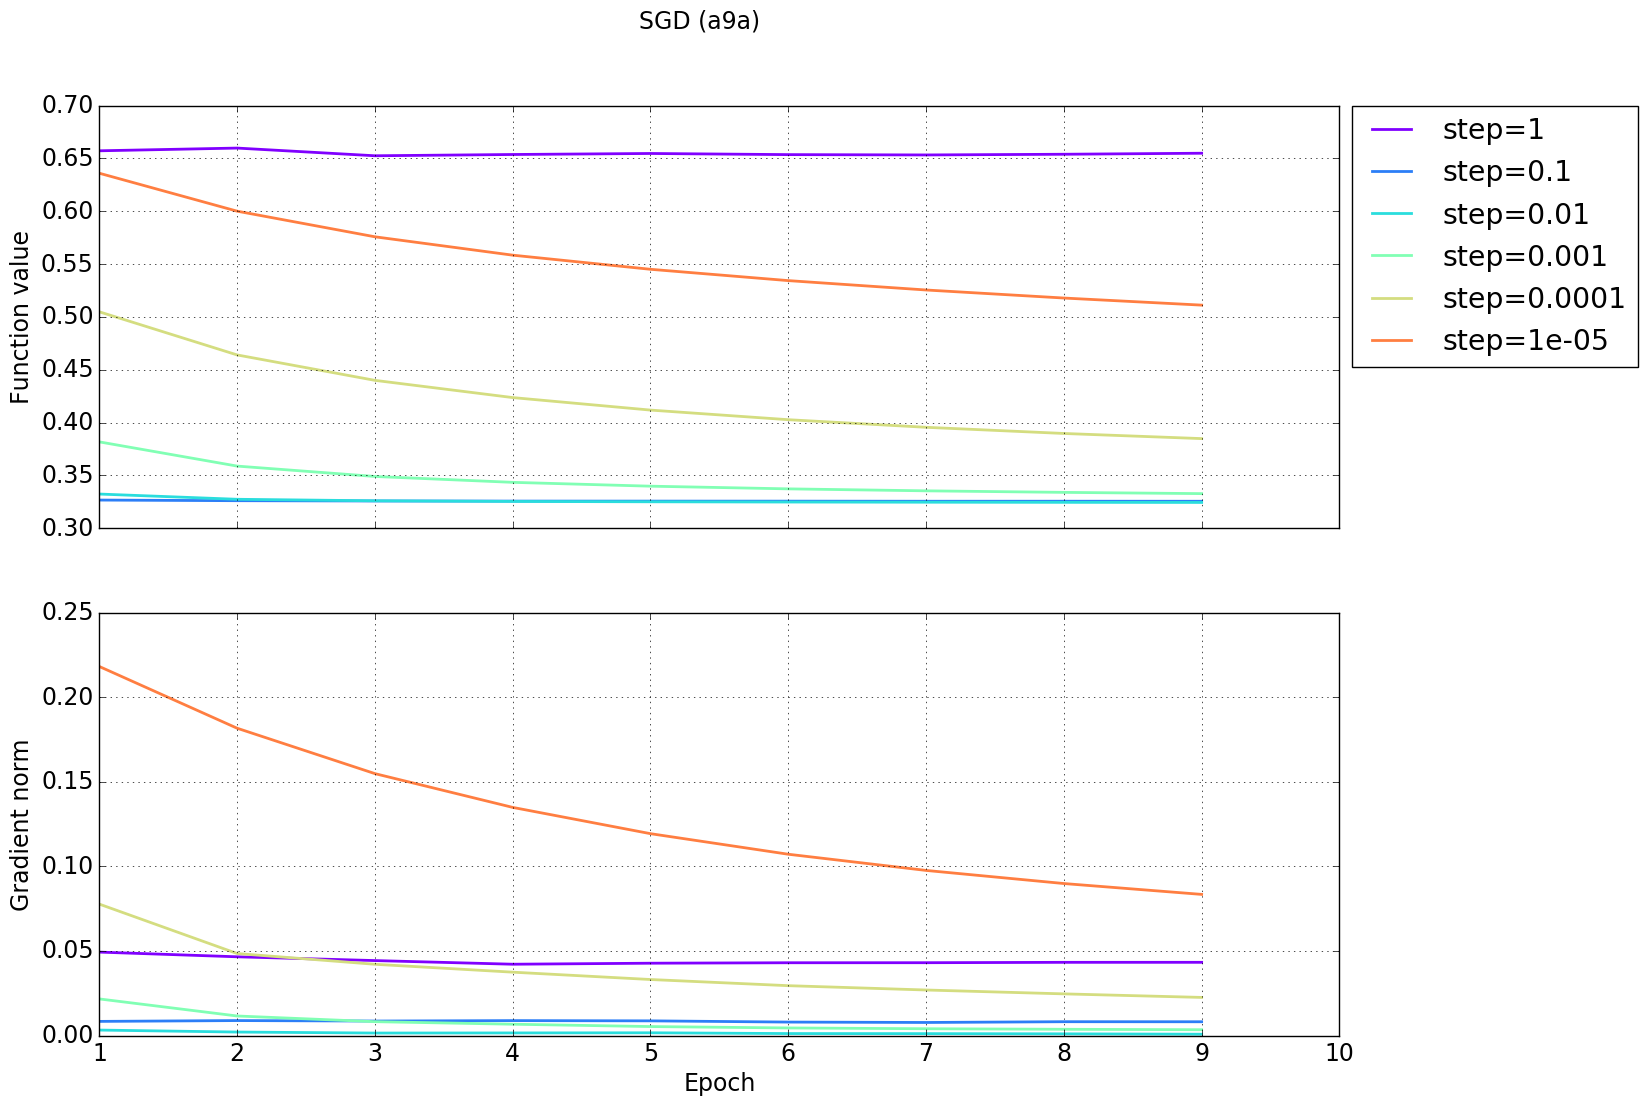
\includegraphics[width=\picwidth]{sgd_a9a.png}\end{center}

    Посмотрим увеличенный вариант. В этом случае, шаг 0.1 показывает хорошие результаты, но метод быстрее при step = 0.01. У нас появился еще один кандидат.

    \begin{center}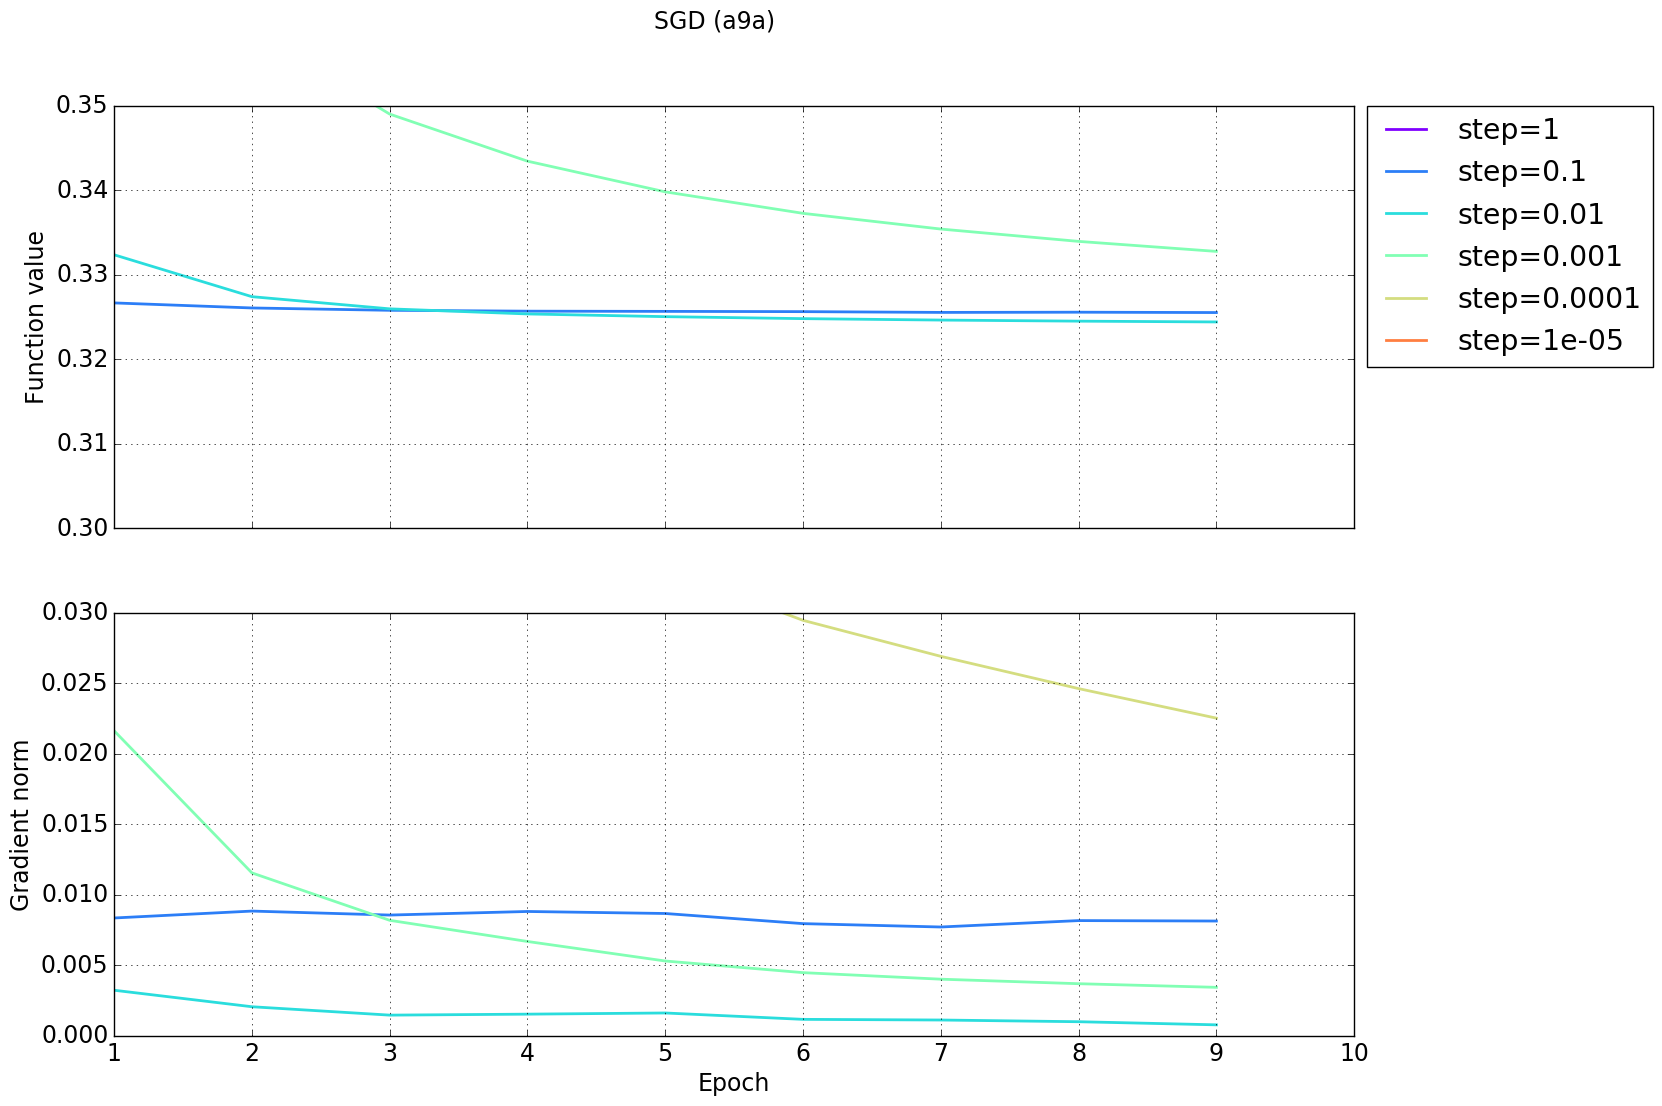
\includegraphics[width=\picwidth]{sgd_a9a_zoomed.png}\end{center}

    Теперь запустим метод для автокодировщика.

    Посмотрим график для атокодировщика с конфигурацией 1. Тут безусловно step = 0.1 показывает лучший результат.

    \begin{center}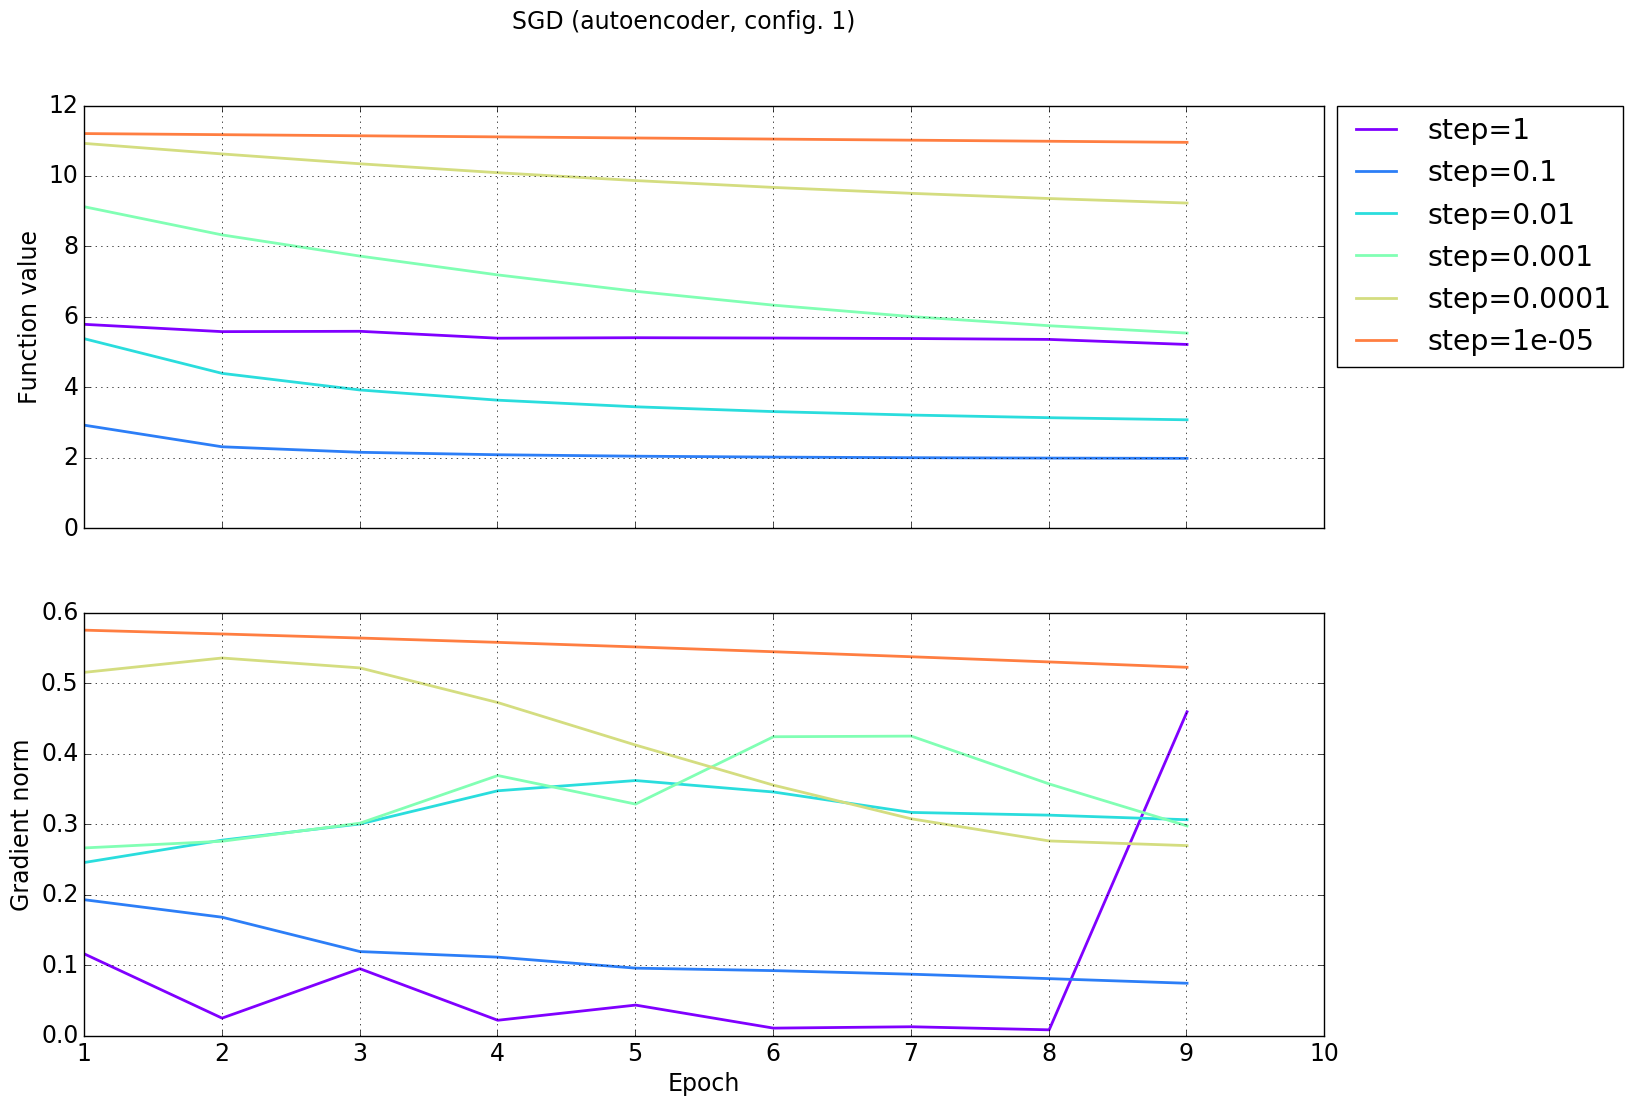
\includegraphics[width=\picwidth]{sgd_autoencoder_conf1.png}\end{center}

    Аналогично и с автокодировщиком с конфигурацией 2.

    \begin{center}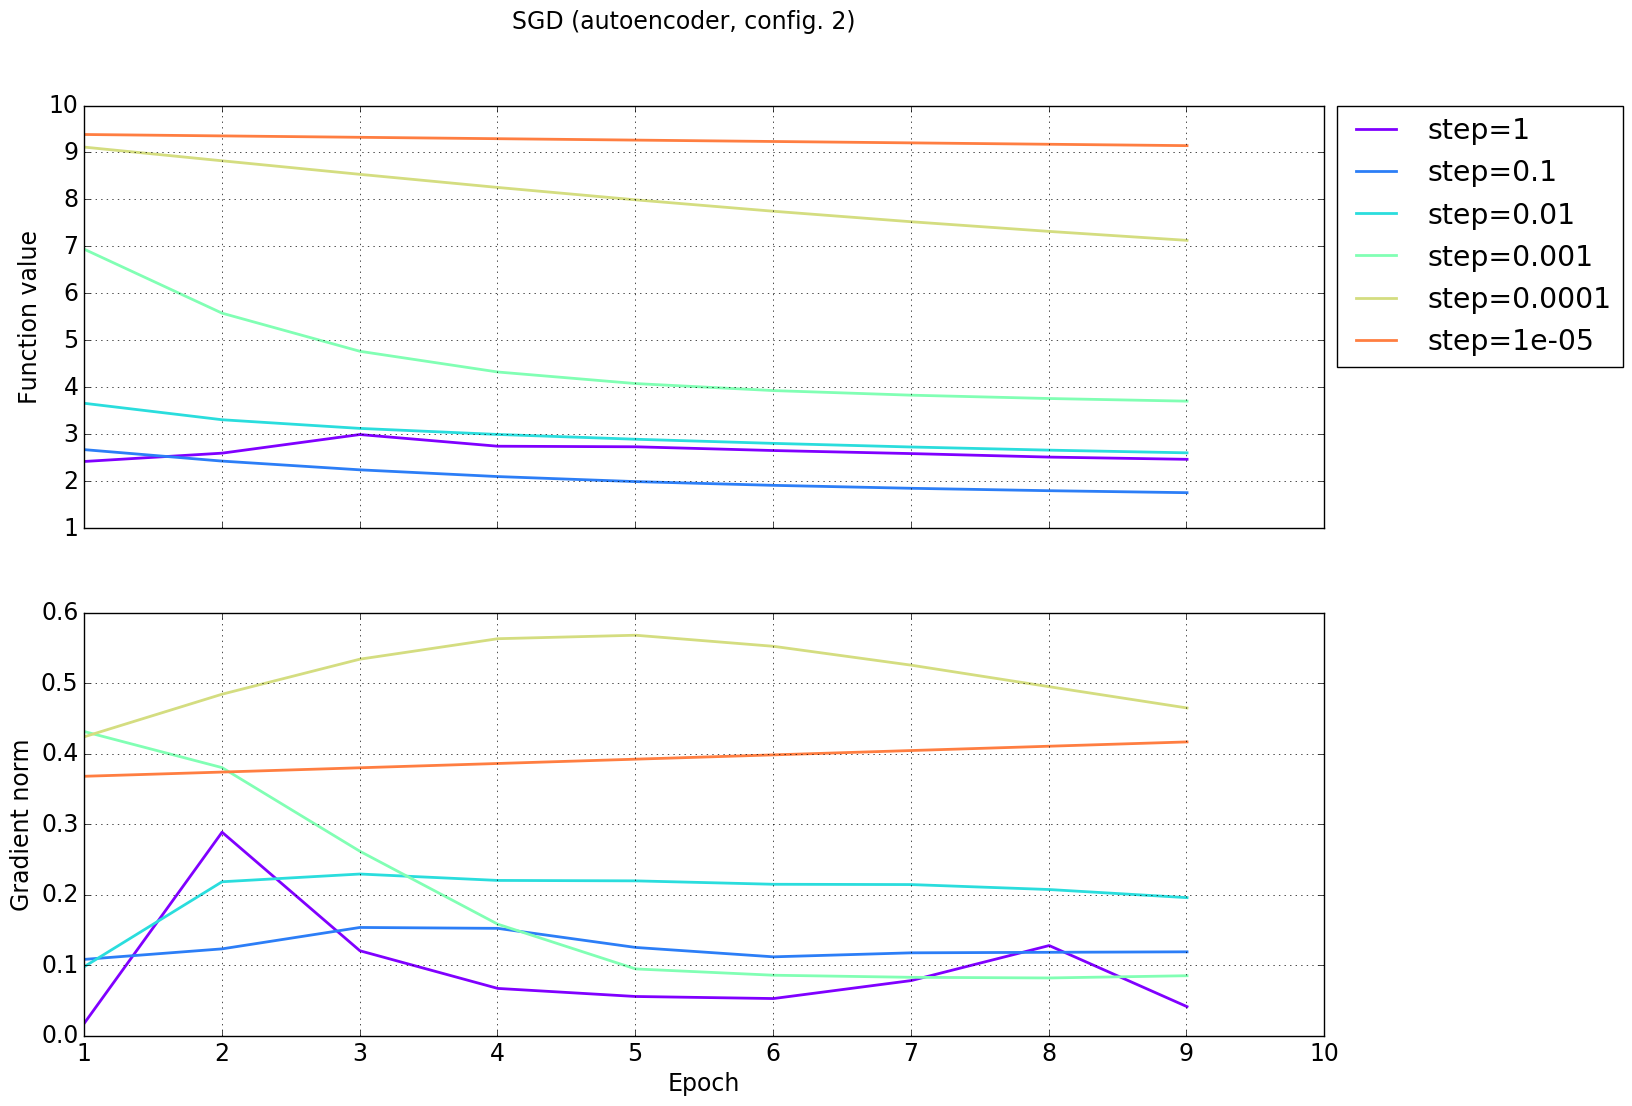
\includegraphics[width=\picwidth]{sgd_autoencoder_conf2.png}\end{center}

    Таким образом, лучшим размером шага, при котором метод сходится быстро является 0.1


    \section{SVRG (Stochastic Variance Reduced Gradient)}
    \subsection{Оптимизация скорости работы SVRG}
    В базовом методе SVRG во внутреннем цикле высчитываются градиенты для случайного $i$ из равномерного распределения. Но при этом, для всех $i \in {1, \dots, n}$ градиенты
    высчитаны во внешнем цикле. Т.е. если мы будем хранить эти градиенты, то вызов оракула во внутреннем цикле не понадобится. Таким образом, мы получаем выигрыш в скорости
    на $O(n)$ ($n$ вызовов оракула). Но при этом мы проигрываем по памяти на $O(n * d)$ ($d$ - размерность пространства). Но считаем, что в памяти мы не ограничены. Результаты
    тестов (тесты были сделаны на данных w5a и a9a) показали, что прирост в скорости 30\%, что является очень хорошим результатом.

    \subsection{Скорость сходимости в зависимости от числа итераций внутреннего цикла}
    Запустим метод для модели логистической регрессии.

    На данных w5a видно, что метод ведет себя примерно одинаково для всех $m$ из теста. Но также видно, что начиная с $m = 2n$, точность не сильно увеличивается,
    но время работы увеличивается достаточно.

    \def \picwidth {17cm}

    \begin{center}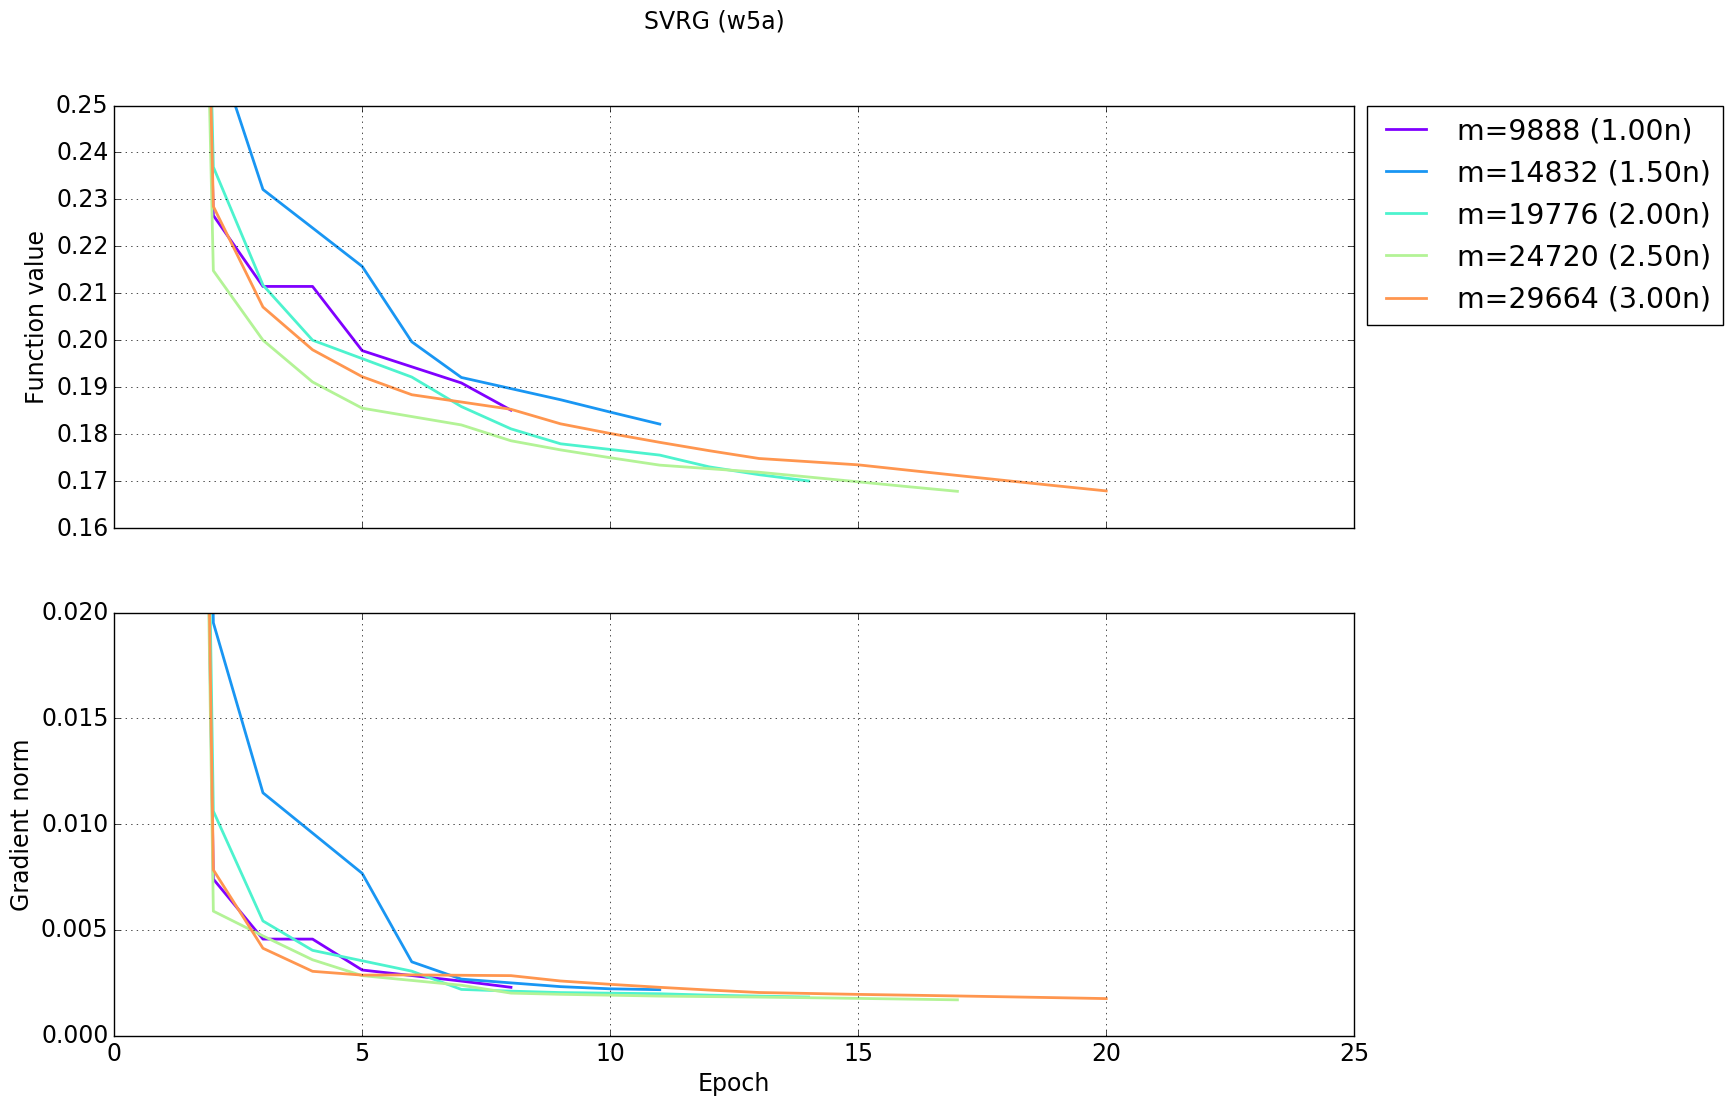
\includegraphics[width=\picwidth]{svrg_w5a_zoomed.png}\end{center}

    Далее посмторим график для данных a9a. Тут примерно тот же случай, что и с w5a.

    \begin{center}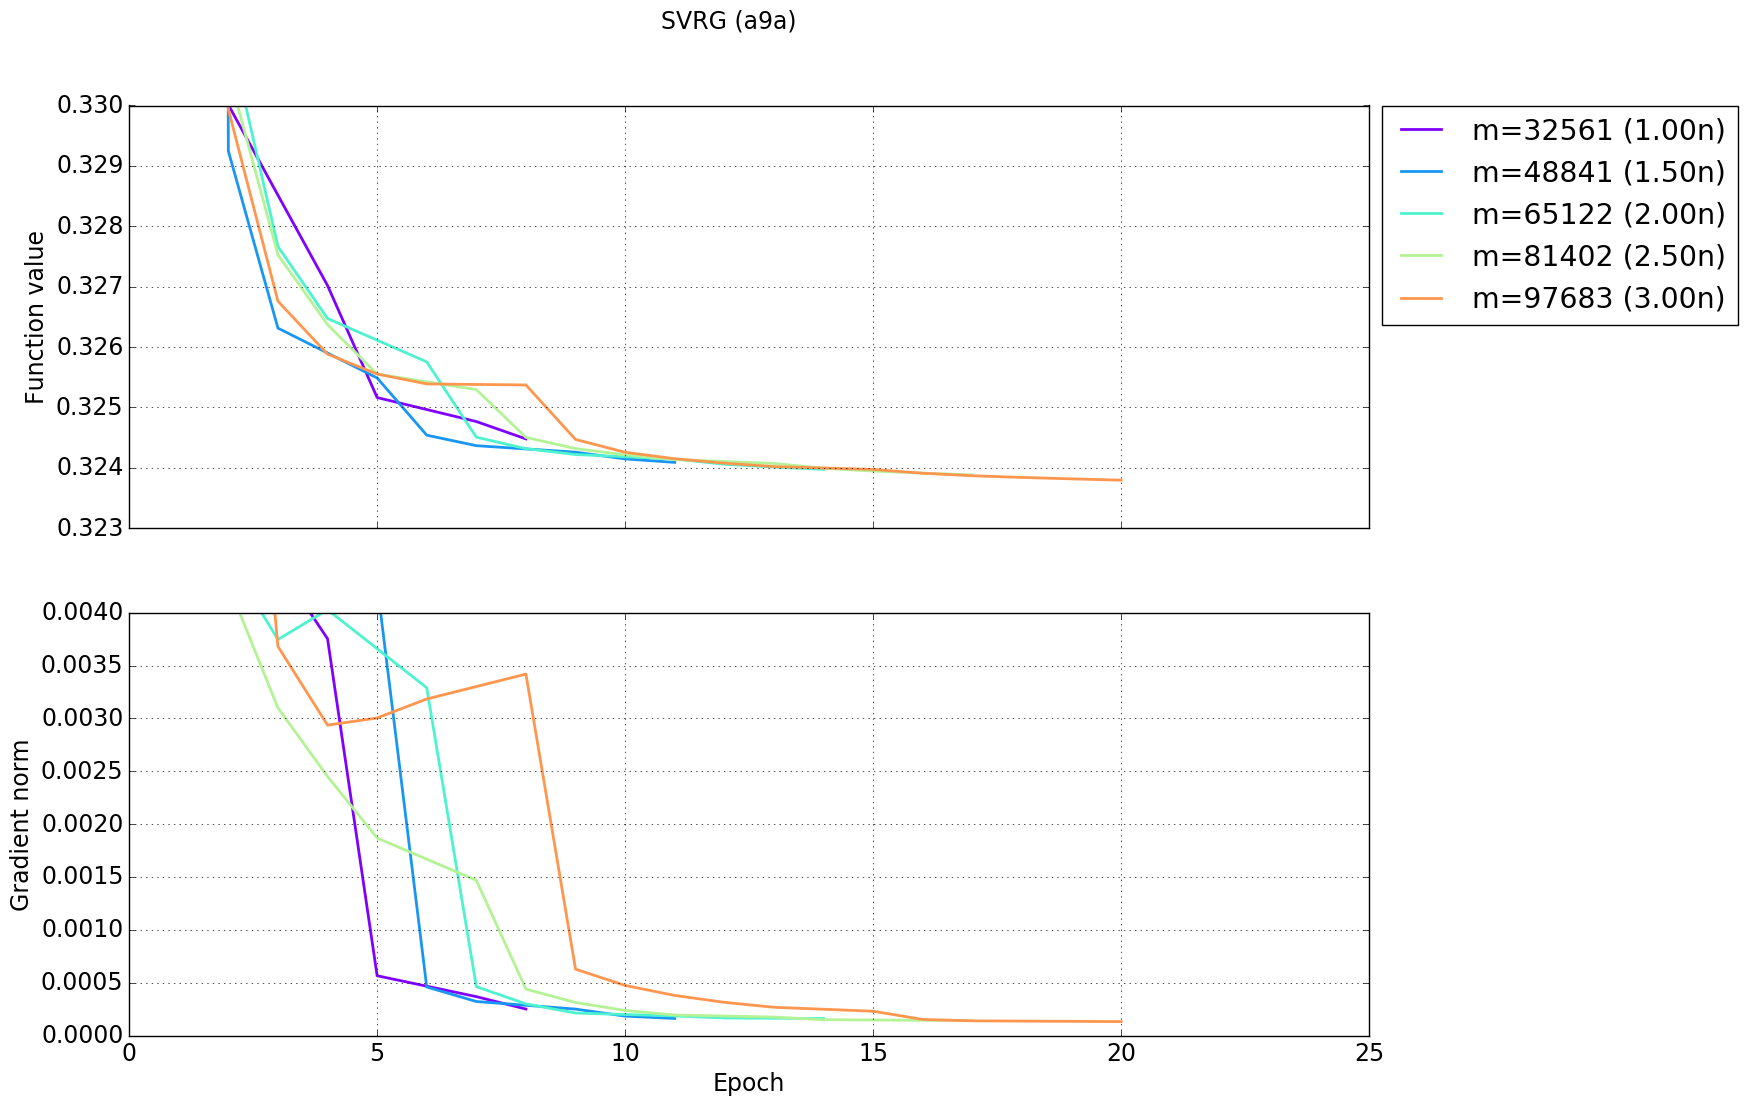
\includegraphics[width=\picwidth]{svrg_a9a_zoomed.png}\end{center}

    Теперь запустим метод для автокодировщика.

    Посмотрим график для атокодировщика с конфигурацией 1 и с конфигурацией 2. Тут ф-ции сходятся также примерно одинаково, но интересен график градиентов.
    Хотя градиент ``скачет'', ф-ции сходятся. Это объсняется тем, что оптимизационная задача автокодировщика не является выпуклой. Такой же эффект можно видеть и для SGD,
    но в случае SGD график более гладкий, потому, что SGD не использует сумму градиентов.

    \begin{center}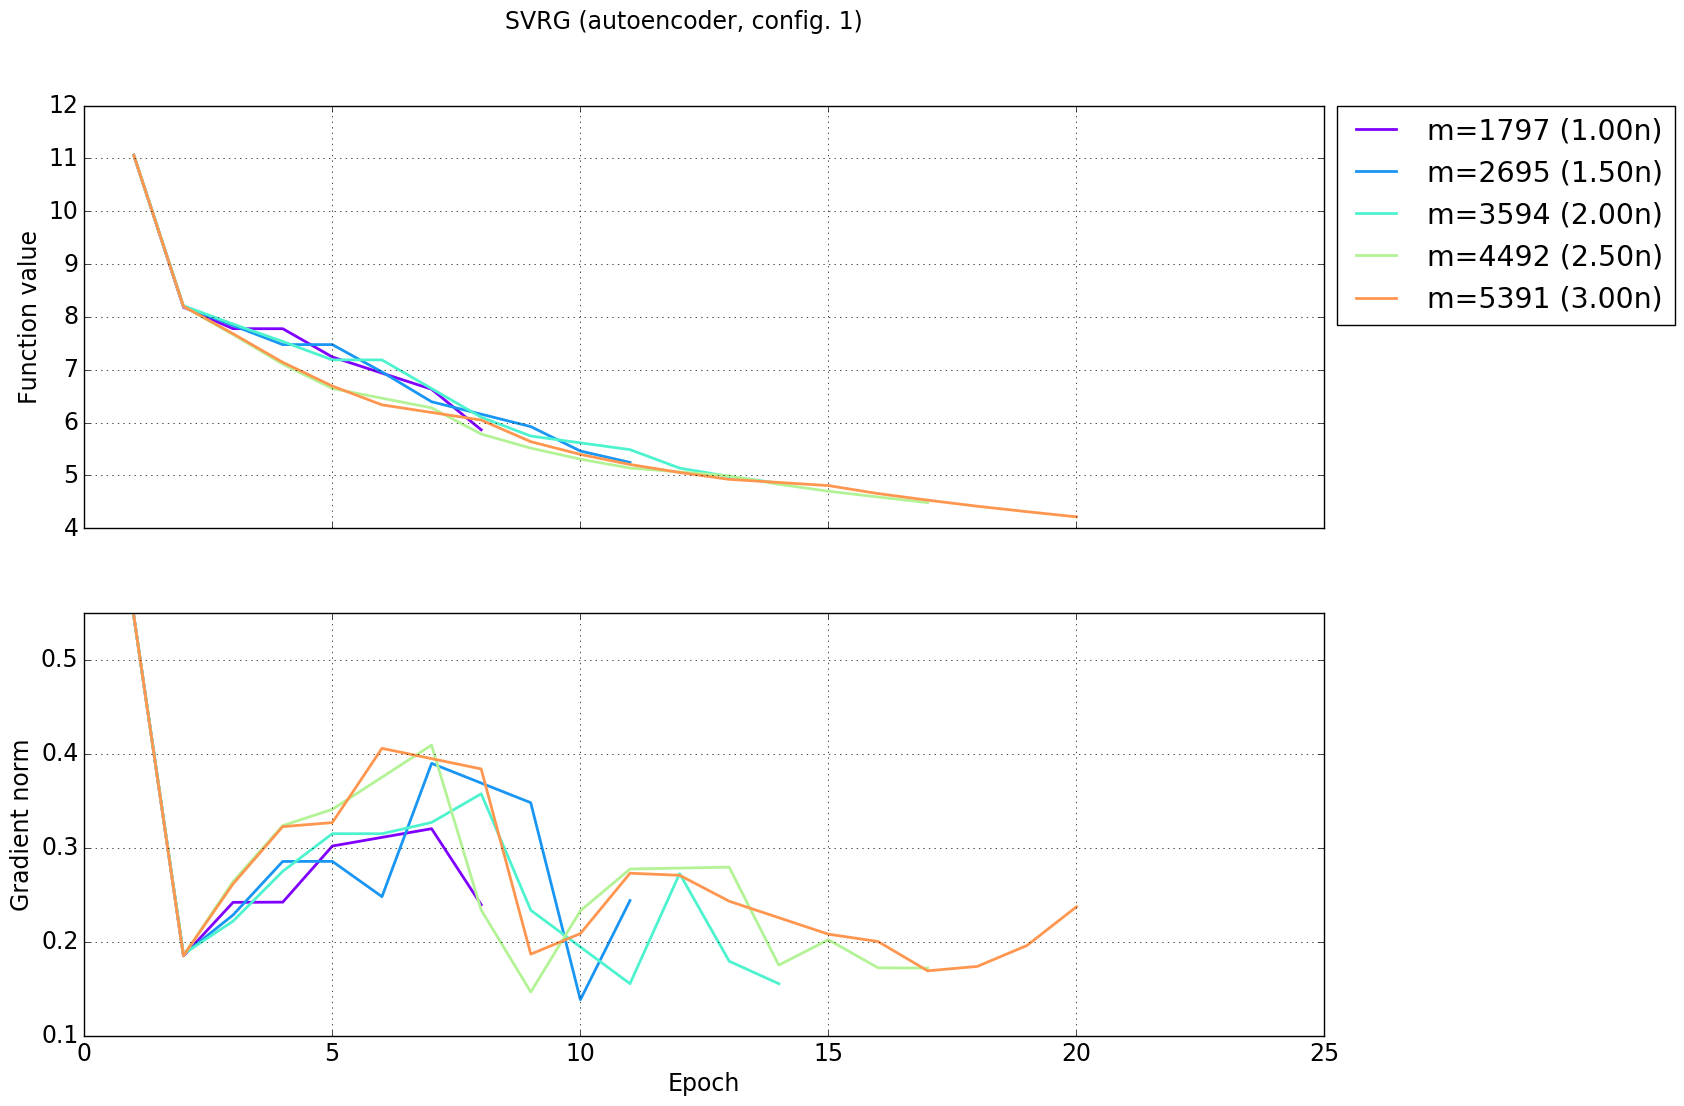
\includegraphics[width=\picwidth]{svrg_autoencoder_conf1.png}\end{center}
    \begin{center}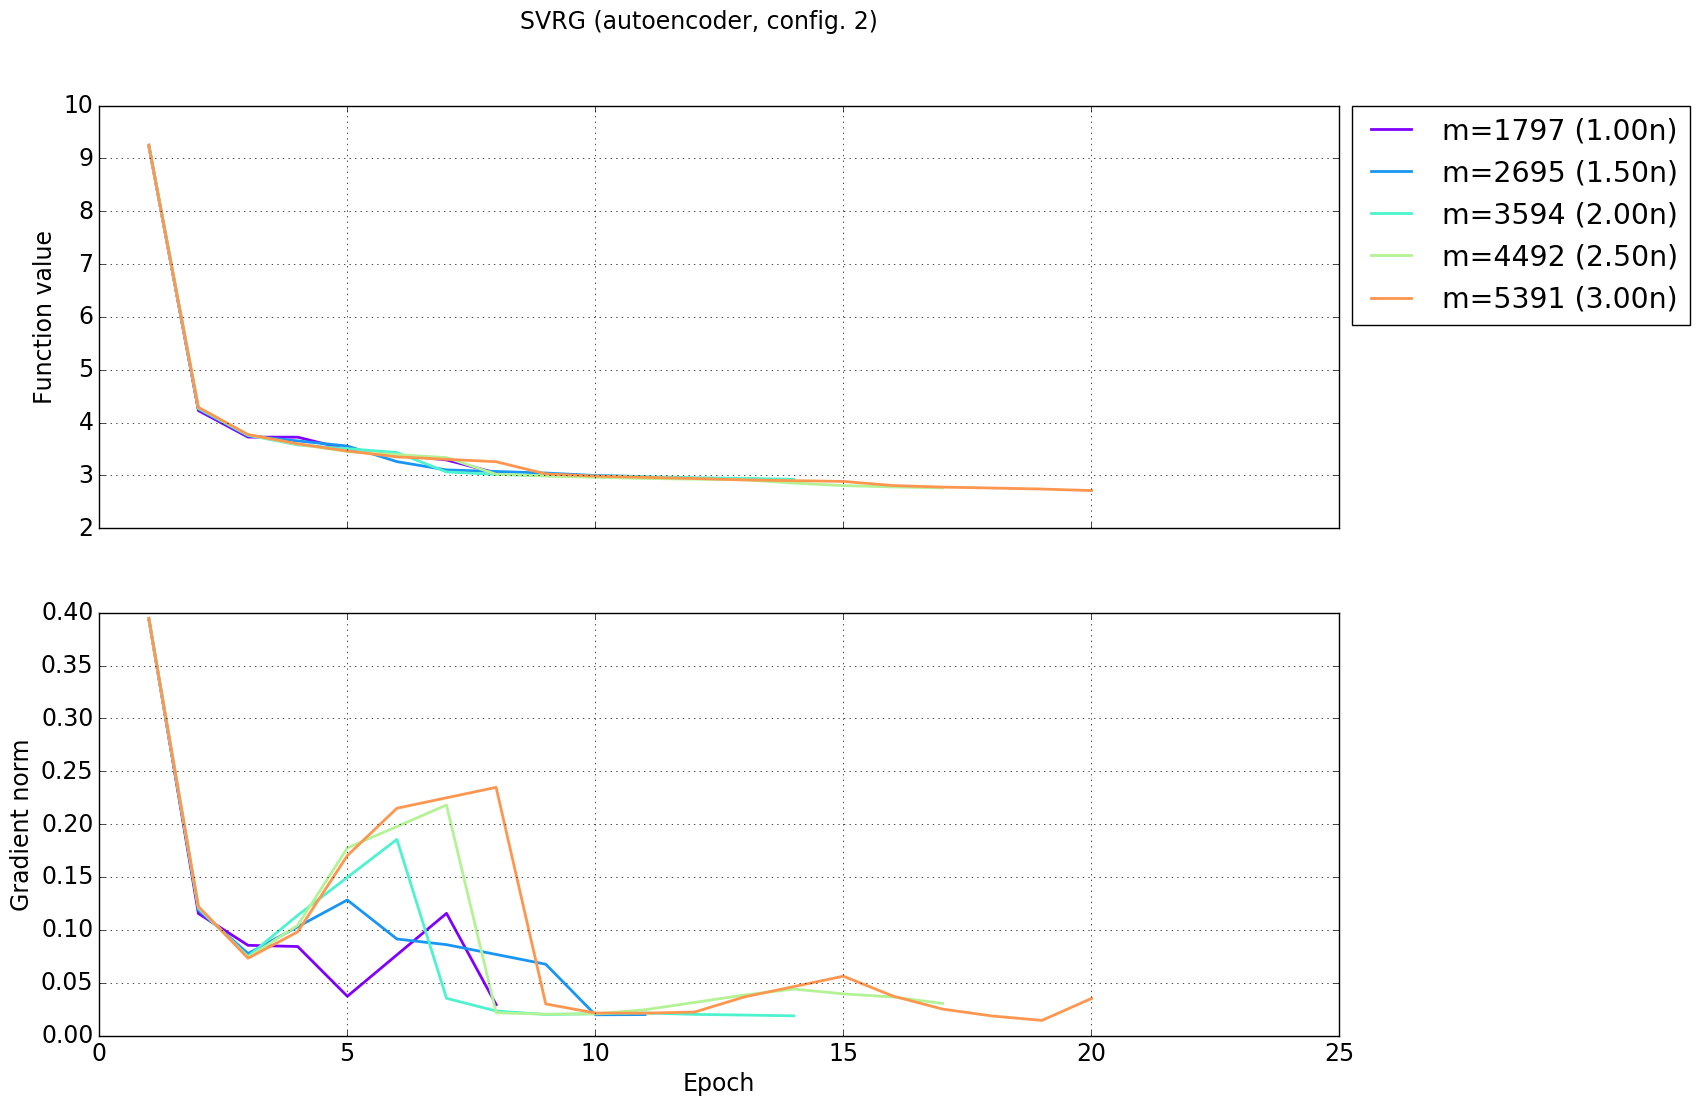
\includegraphics[width=\picwidth]{svrg_autoencoder_conf2.png}\end{center}

    Таким образом, число нутренних итераций выбирется равным $2n$ (где $n$ - число функций).

    \section{Сравнение SGD и SVRG}
    Параметры SGD: длина шага = 0.1; количество итераций $20n$

    Параметры SVRG: число стадий 10

    Сперва сравним методы на задаче логистической регрессии.

    Хорошо видно, что на данных w5a метод SVRG не может достичь минимума SGD даже проделав больее чем в два раза больше эпох. Хотя теоретически, SVRG должен работать лучше.
    Допустим, что это из-за данных и сравним методы на данных a9a.

    \begin{center}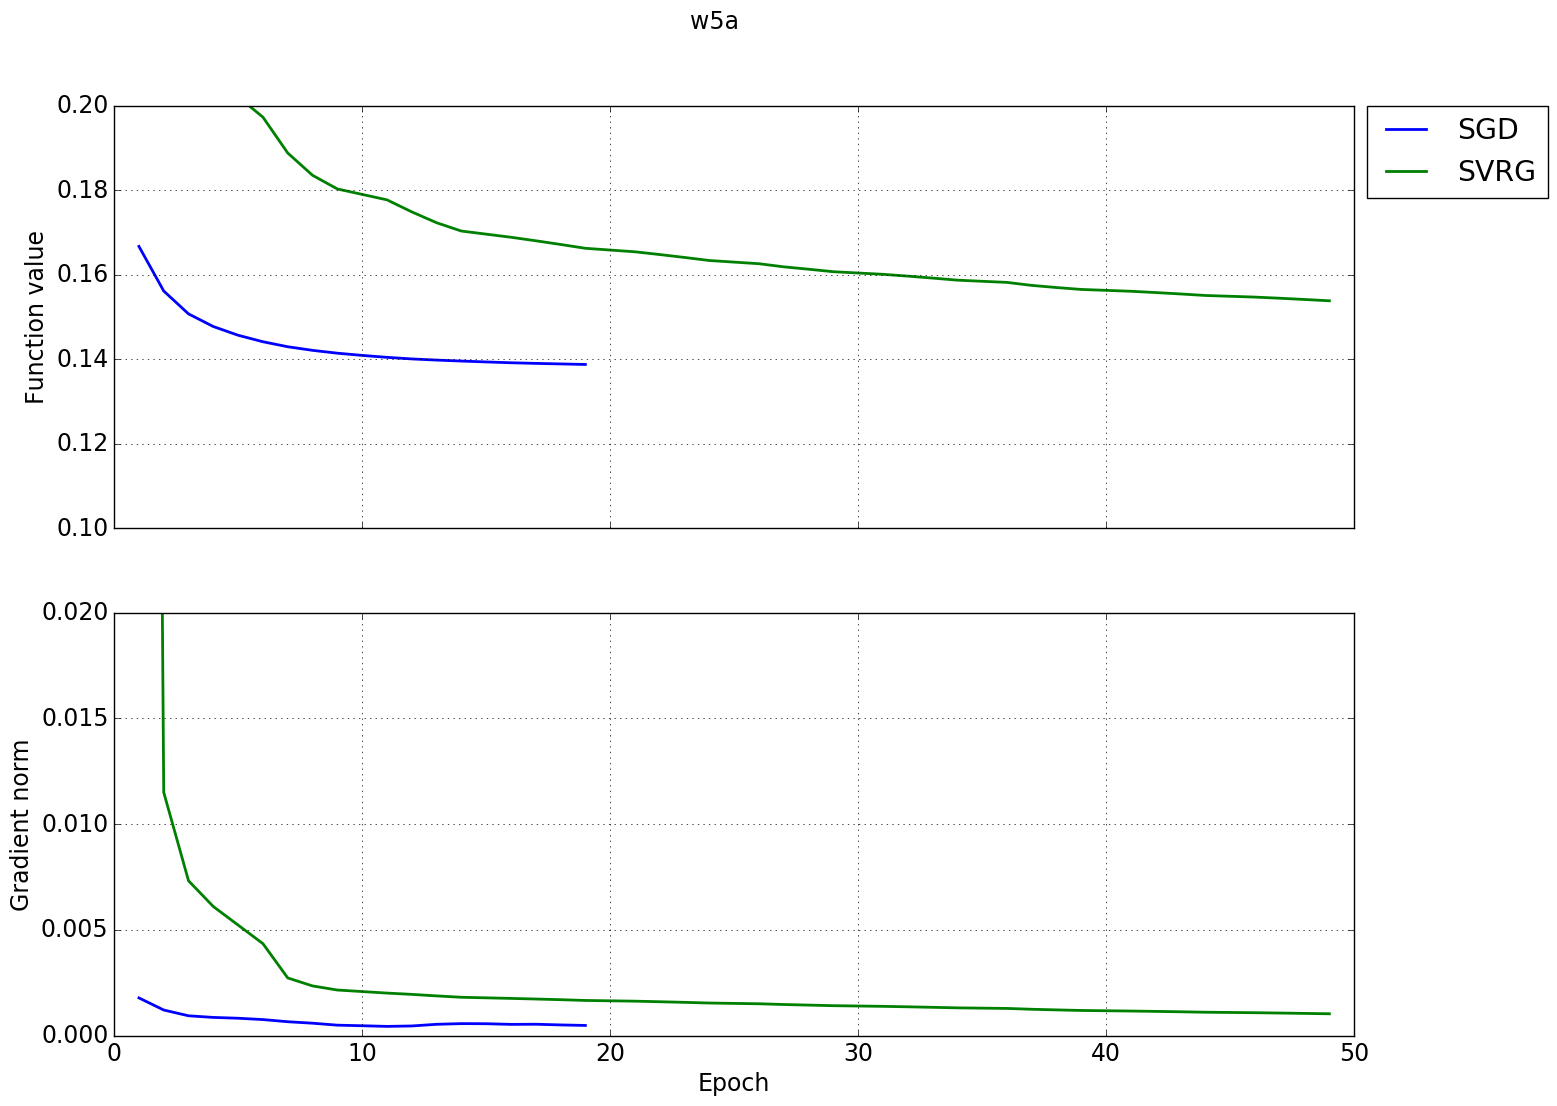
\includegraphics[width=\picwidth]{cmp_w5a.png}\end{center}

    На данных a9a вроде бы все хорошо и SVRG работает лучше.

    \begin{center}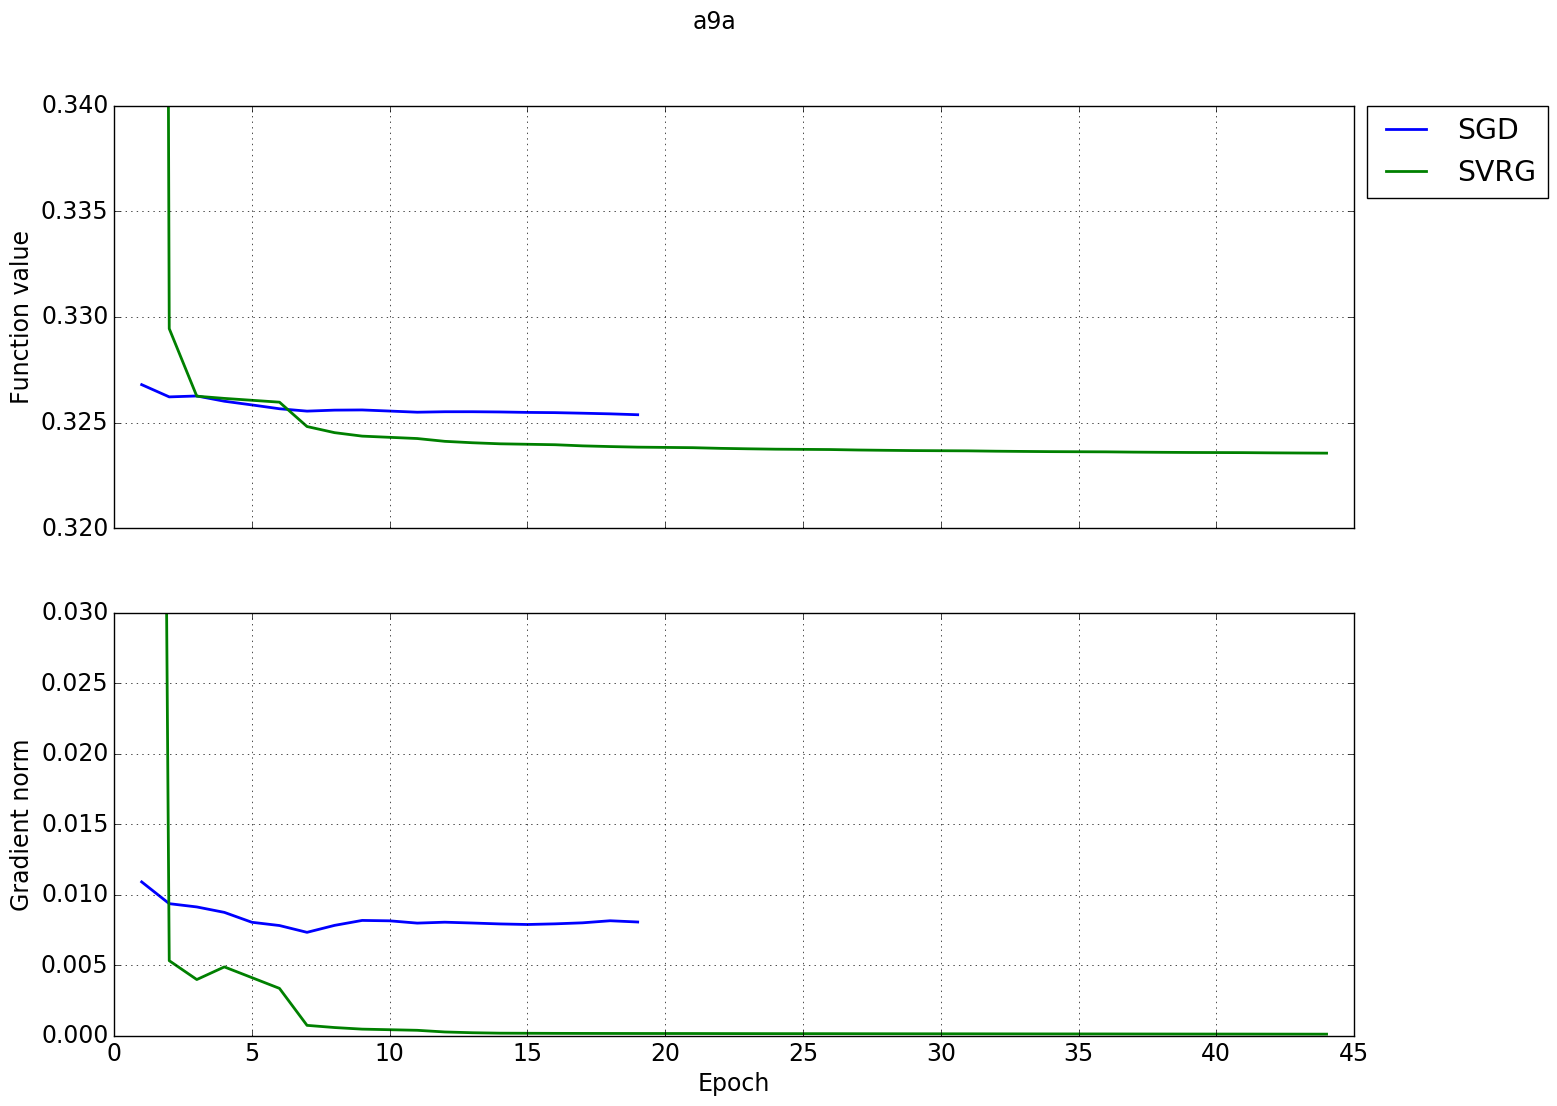
\includegraphics[width=\picwidth]{cmp_a9a.png}\end{center}

    Но почему на w5a SVRG работает хуже SGD? Может из-за выбора шага? Давайте проверим, поставив шаг равным константе 0.1. Т.е. L = 1 (число стадий 3)

    На графиках видно, что SVRG все таки быстрее сходится и даже ``проваливается'' ниже SGD. Но почему метод Нестерова работает не так хорошо, как хотелось бы?
    Ответ на этот вопрос пока остается загадкой =)
    \begin{center}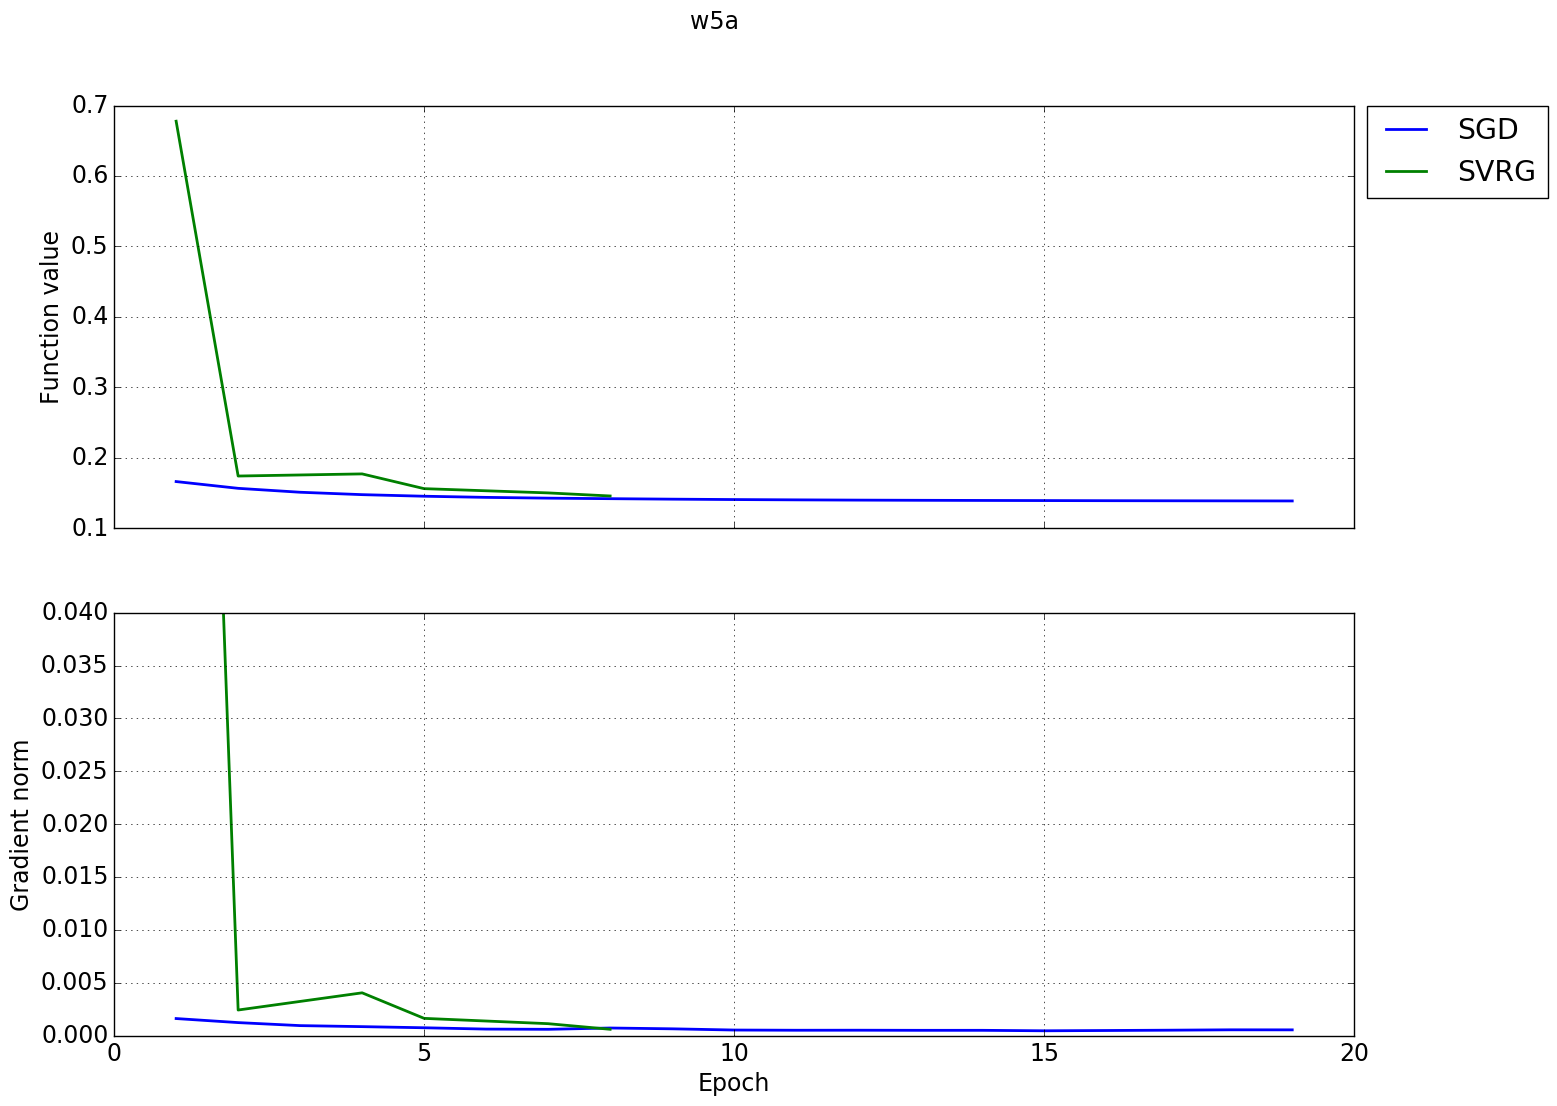
\includegraphics[width=\picwidth]{cmp_w5a_fix_step.png}\end{center}
    \begin{center}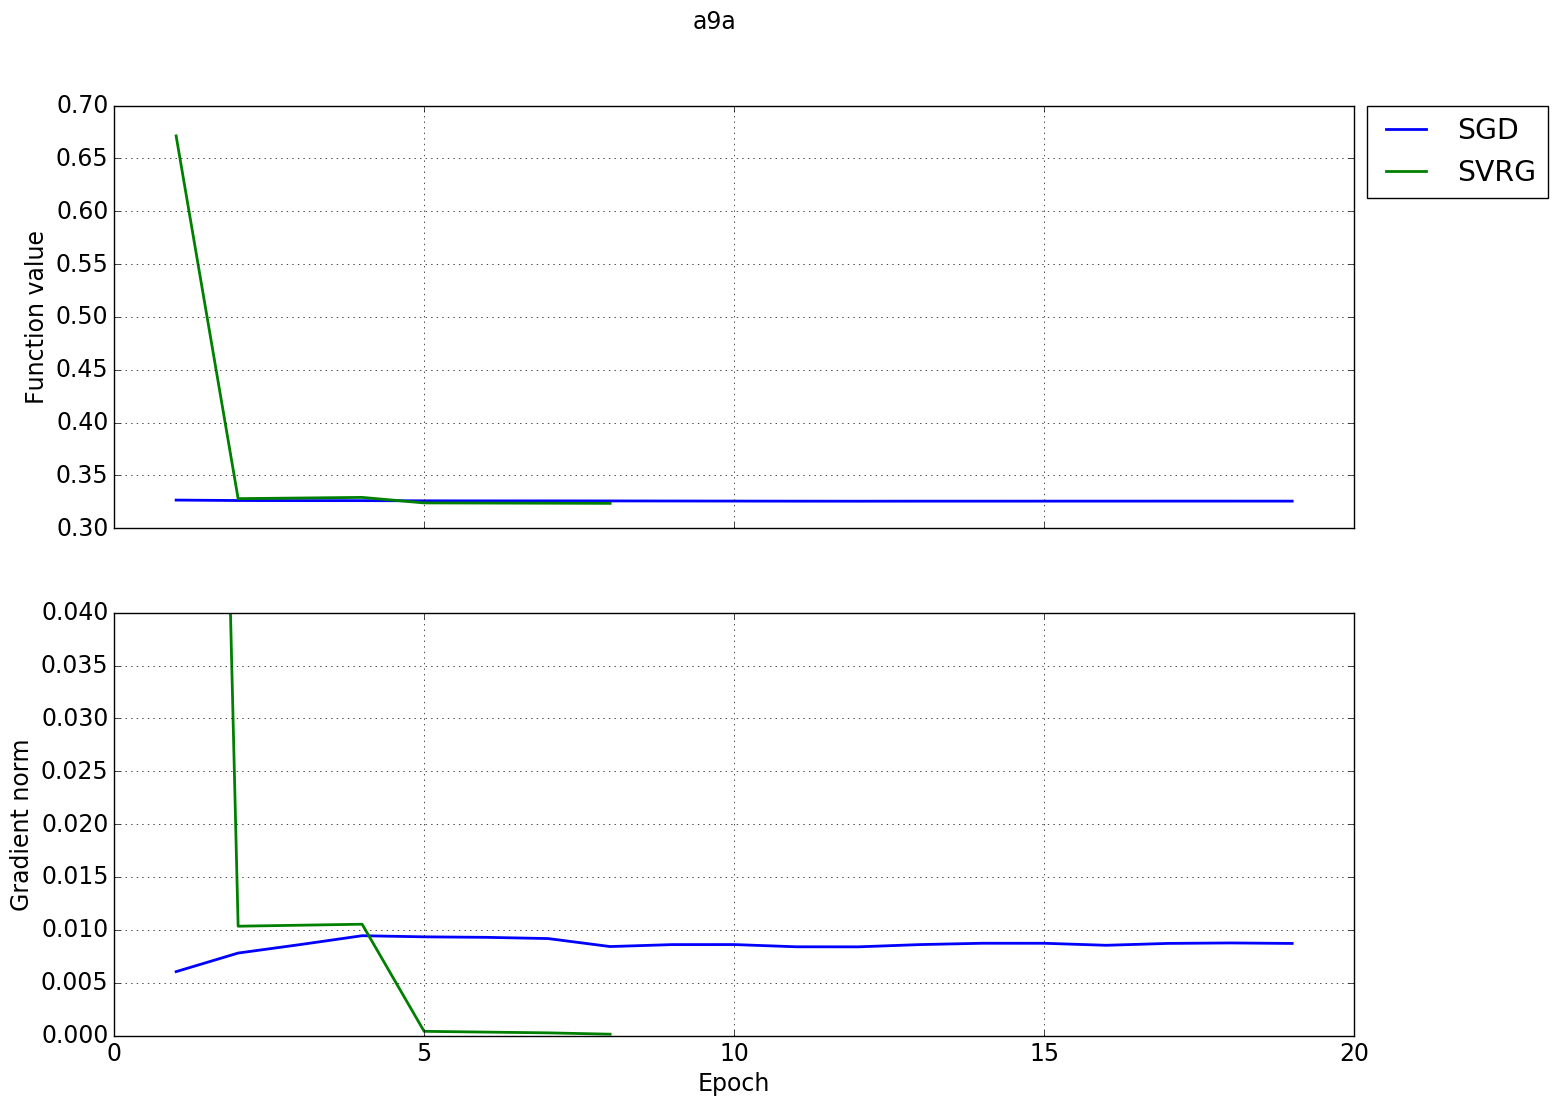
\includegraphics[width=\picwidth]{cmp_a9a_fix_step.png}\end{center}

    Теперь посмотрим сравнение скоростей для автокодировщика.

    Тут SVRG никак не лучше SGD, и скорее всего это из-за эмпирического подбора шага.

    \begin{center}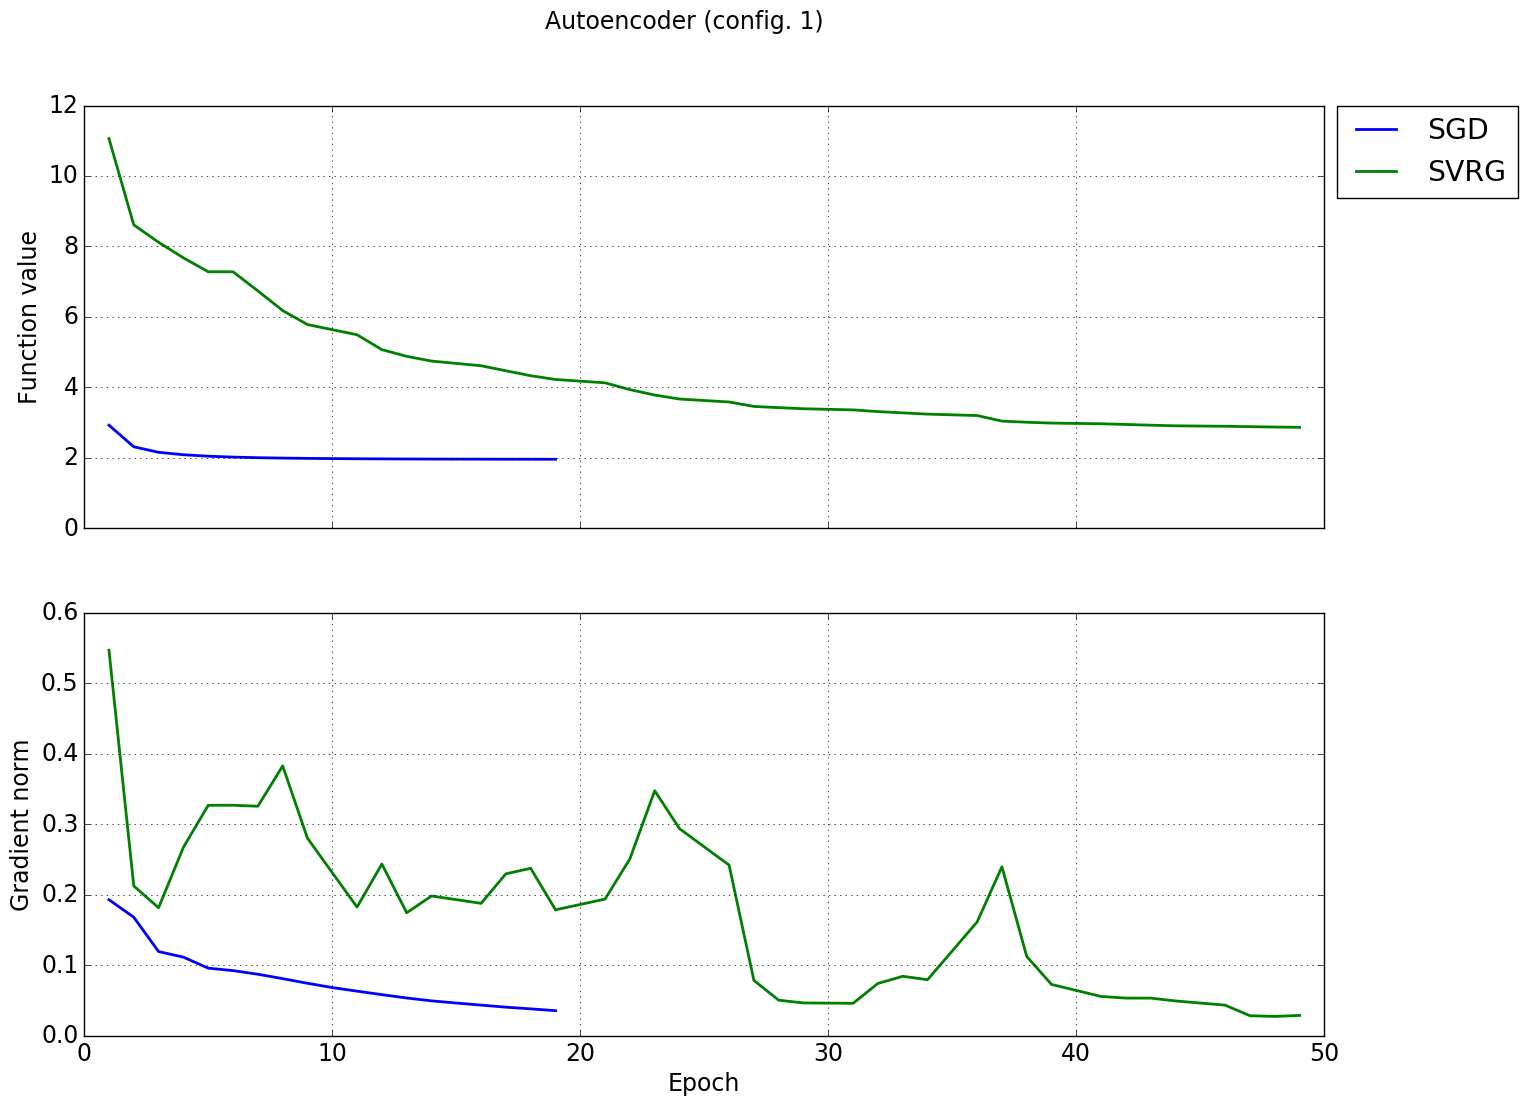
\includegraphics[width=\picwidth]{cmp_ae1.png}\end{center}
    \begin{center}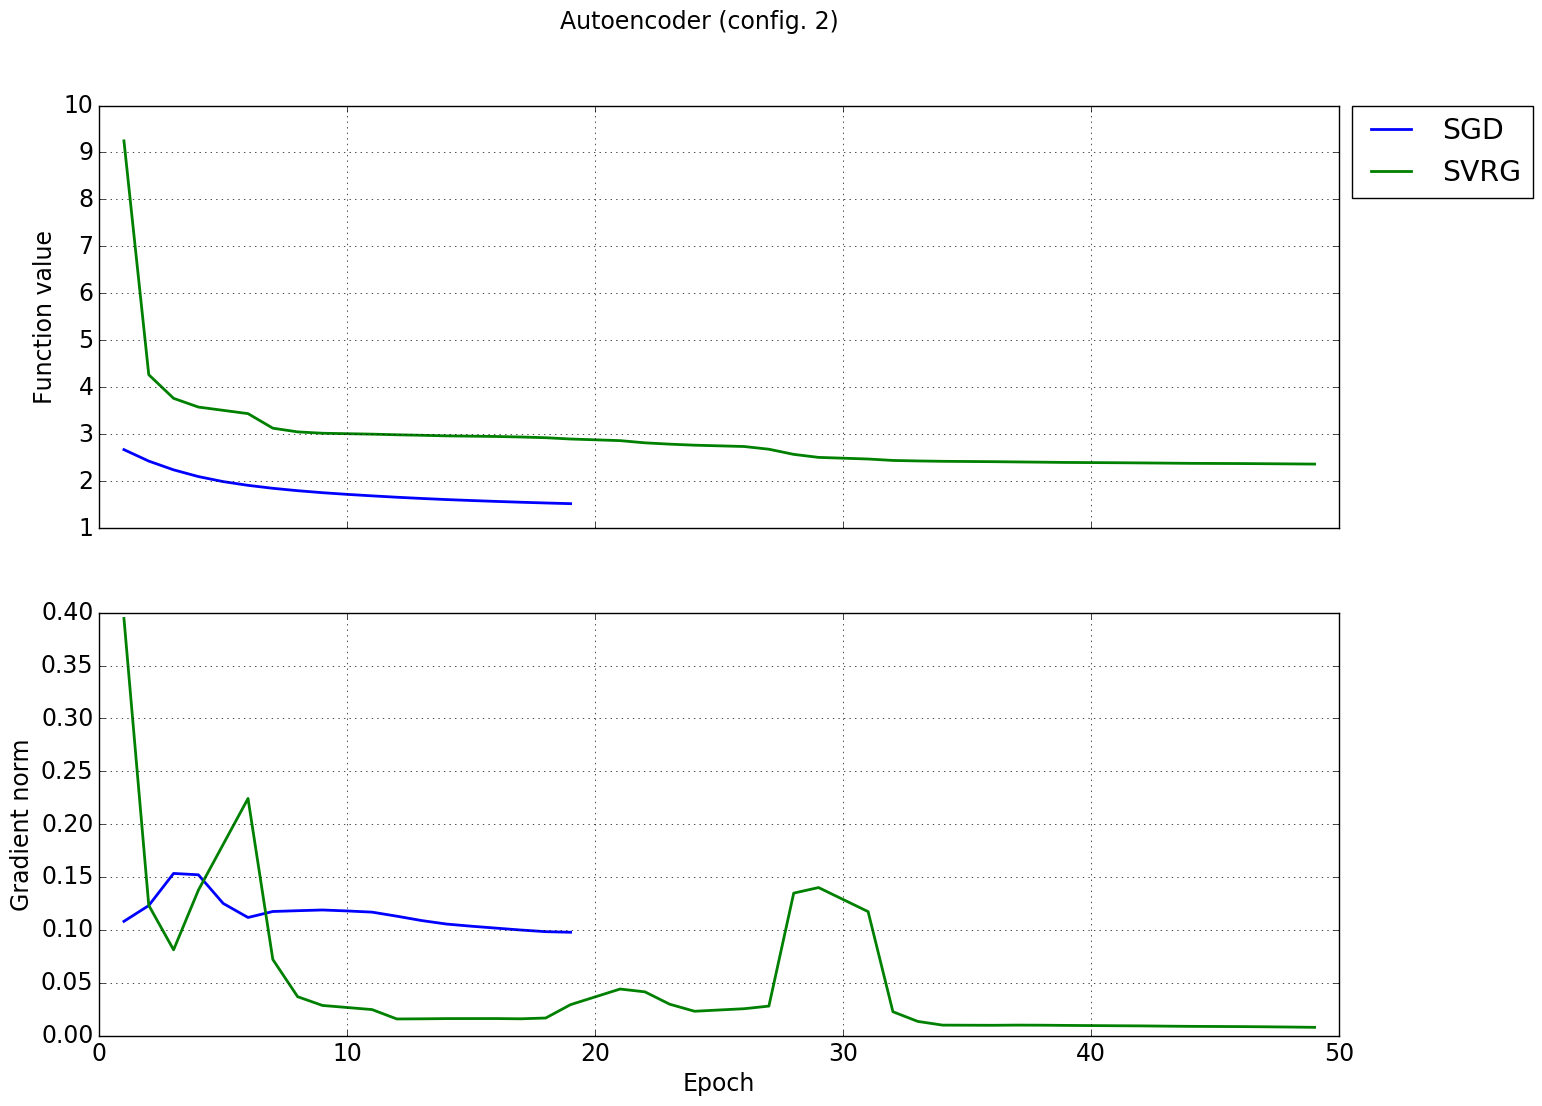
\includegraphics[width=\picwidth]{cmp_ae2.png}\end{center}

    Также, разница между работой SGD и SVRG видна на результатах работы двух методов:

    \begin{center}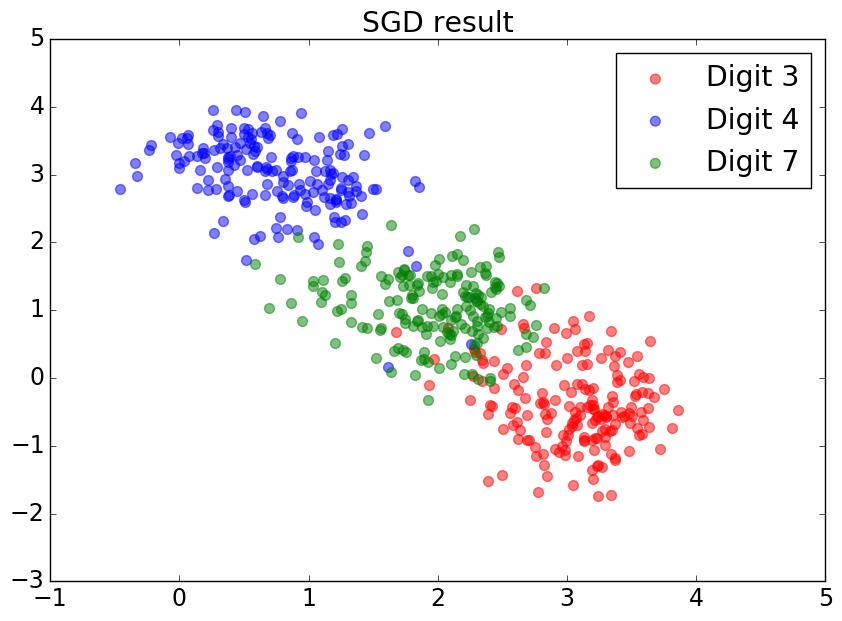
\includegraphics[width=\picwidth]{proj_sgd.png}\end{center}
    \begin{center}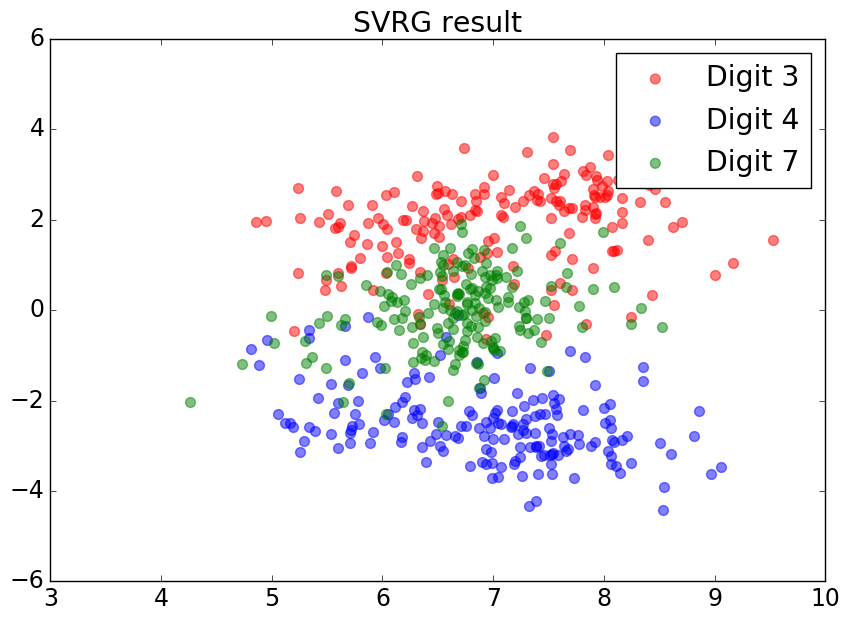
\includegraphics[width=\picwidth]{proj_svrg.png}\end{center}

    \section{Заключение}
    В работе были исследованы методы SVRG и SGD и получены следующие результаты:
    \begin{enumerate}
        \item Метод SGD бысрее сходится, чем SVRG с подбором шага по методу Нестерова.
        \item Метод SGD бысрее и точнее сходится при размере шага = 0.1.
        \item Метод SVRG с постоянным размером шага бысрее сходится, чем SGD.
        \item Метод SVRG бысрее и точнее сходится при количестве внутренних итераций равному $2n$.
        \item Метод SVRG работает быстрее, если сохранять градиенты во внешнем цикле.
        \item Метод SVRG с постоянным размером шага бысрее сходится, чем SVRG с эмпирическим подбором шага.
    \end{enumerate}

\end{document}
